%\documentclass{article}
%\usepackage{graphicx,subfigure}
%\begin{document}

\begin{figure}[h]
  \centering
   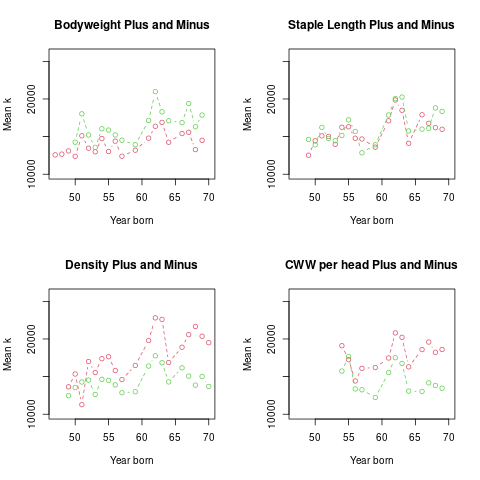
\includegraphics[width=1.4\textwidth,height=1.7\textwidth]{ab1fs/kfs2.png}
	\caption{Data from Turner, Brooker, and Dolling (1970)~\cite{turn:70} showing the mean $k$ value for sheep born in years 1947 to 1970  of four single trait selection lines with selection up and down for eight wool traits. Red lines are Plus selection. Green lines are Minus selection}
  \label{fig:kfs2}
\end{figure}

%\end{document}

